\section{Side by side comparison between analysis results}
\label{sec:sidebyside}

\begin{table}[H]
    \begin{minipage}{.4\textwidth}
    \begin{table}[H]
    \centering
    \small
    \begin{tabular}{|c|c|c|c|}
          \hline
          Node/Branch & $@(i) [A]/ v [V]$\\
          \hline
          @cb[i] & 0.000000e+00\\ \hline
@ce[i] & 0.000000e+00\\ \hline
@q1[ib] & 7.022567e-05\\ \hline
@q1[ic] & 1.404513e-02\\ \hline
@q1[ie] & -1.41154e-02\\ \hline
@q1[is] & 5.765392e-12\\ \hline
@rc[i] & 1.411536e-02\\ \hline
@re[i] & 1.411536e-02\\ \hline
@rf[i] & 7.022567e-05\\ \hline
@rs[i] & 0.000000e+00\\ \hline
v(1) & 0.000000e+00\\ \hline
v(2) & 0.000000e+00\\ \hline
base & 2.254108e+00\\ \hline
coll & 5.765392e+00\\ \hline
emit & 1.411536e+00\\ \hline
vcc & 1.000000e+01\\ \hline

          \hline
    \end{tabular}
    \caption{Solution from simulation.}
    \label{tab:ngs_tau}
    \end{table}
    \end{minipage}
    \begin{minipage}{.29\textwidth}
      \centering
      \begin{tabular}{c|c}
        \hline
          Branch &  Current (A) \\
          \hline
          \input{"currents_branches_first_alienea.tex"}
          \hline
      \end{tabular}
    \label{tab:current2}
    \caption{Currents from theoretical solution}
    \end{minipage}
    \begin{minipage}{.29\textwidth}
      \begin{equation} \Vec{b} = \begin{bmatrix}  5.0385\\  4.7582\\  4.1705\\      -0\\  4.7985\\  5.6468\\ -1.8345\\ -2.7568 \end{bmatrix} \label{eqsol} \end{equation}
      \caption{Voltages from theoretical solution}
      \end{minipage}
    \caption{Solution for voltages for all nodes and current for all branches for $t<0$.}
    \end{table}

The only difference found between the 2 solutions, for the digits presetned here are for $V_3$ and $V_6$, but only in the last digit presented, meaning a difference around $10^{-6} V$. Differences that are probably result of numerical errors, rather than real differences in solutions.

\begin{figure}[H]
\hspace{-10mm}
  \subfigure[Theoretical analysis]{% 
    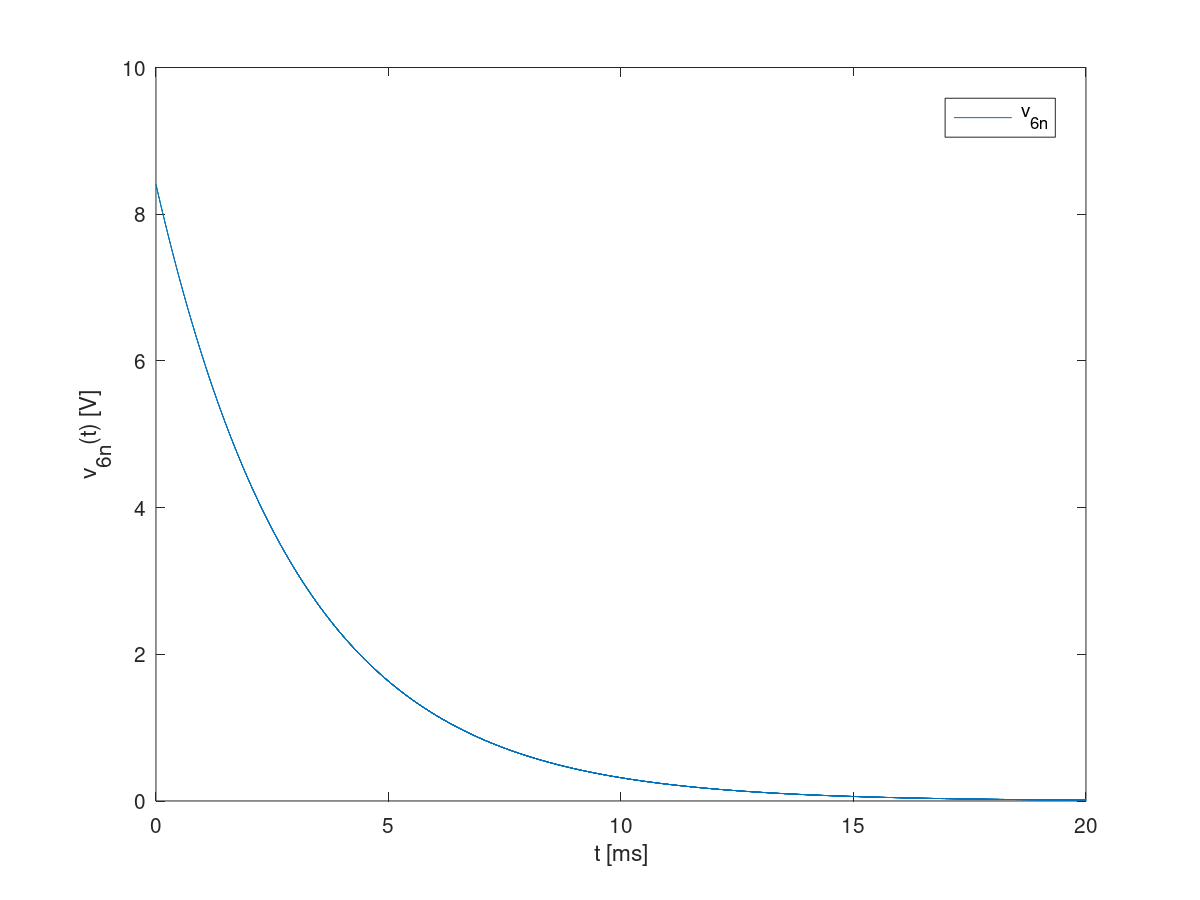
\includegraphics[width=.6\textwidth]{../mat/v6n.png} \label{fig:teo_nat} 
  } 
  \subfigure[Simulation analysis]{% 
    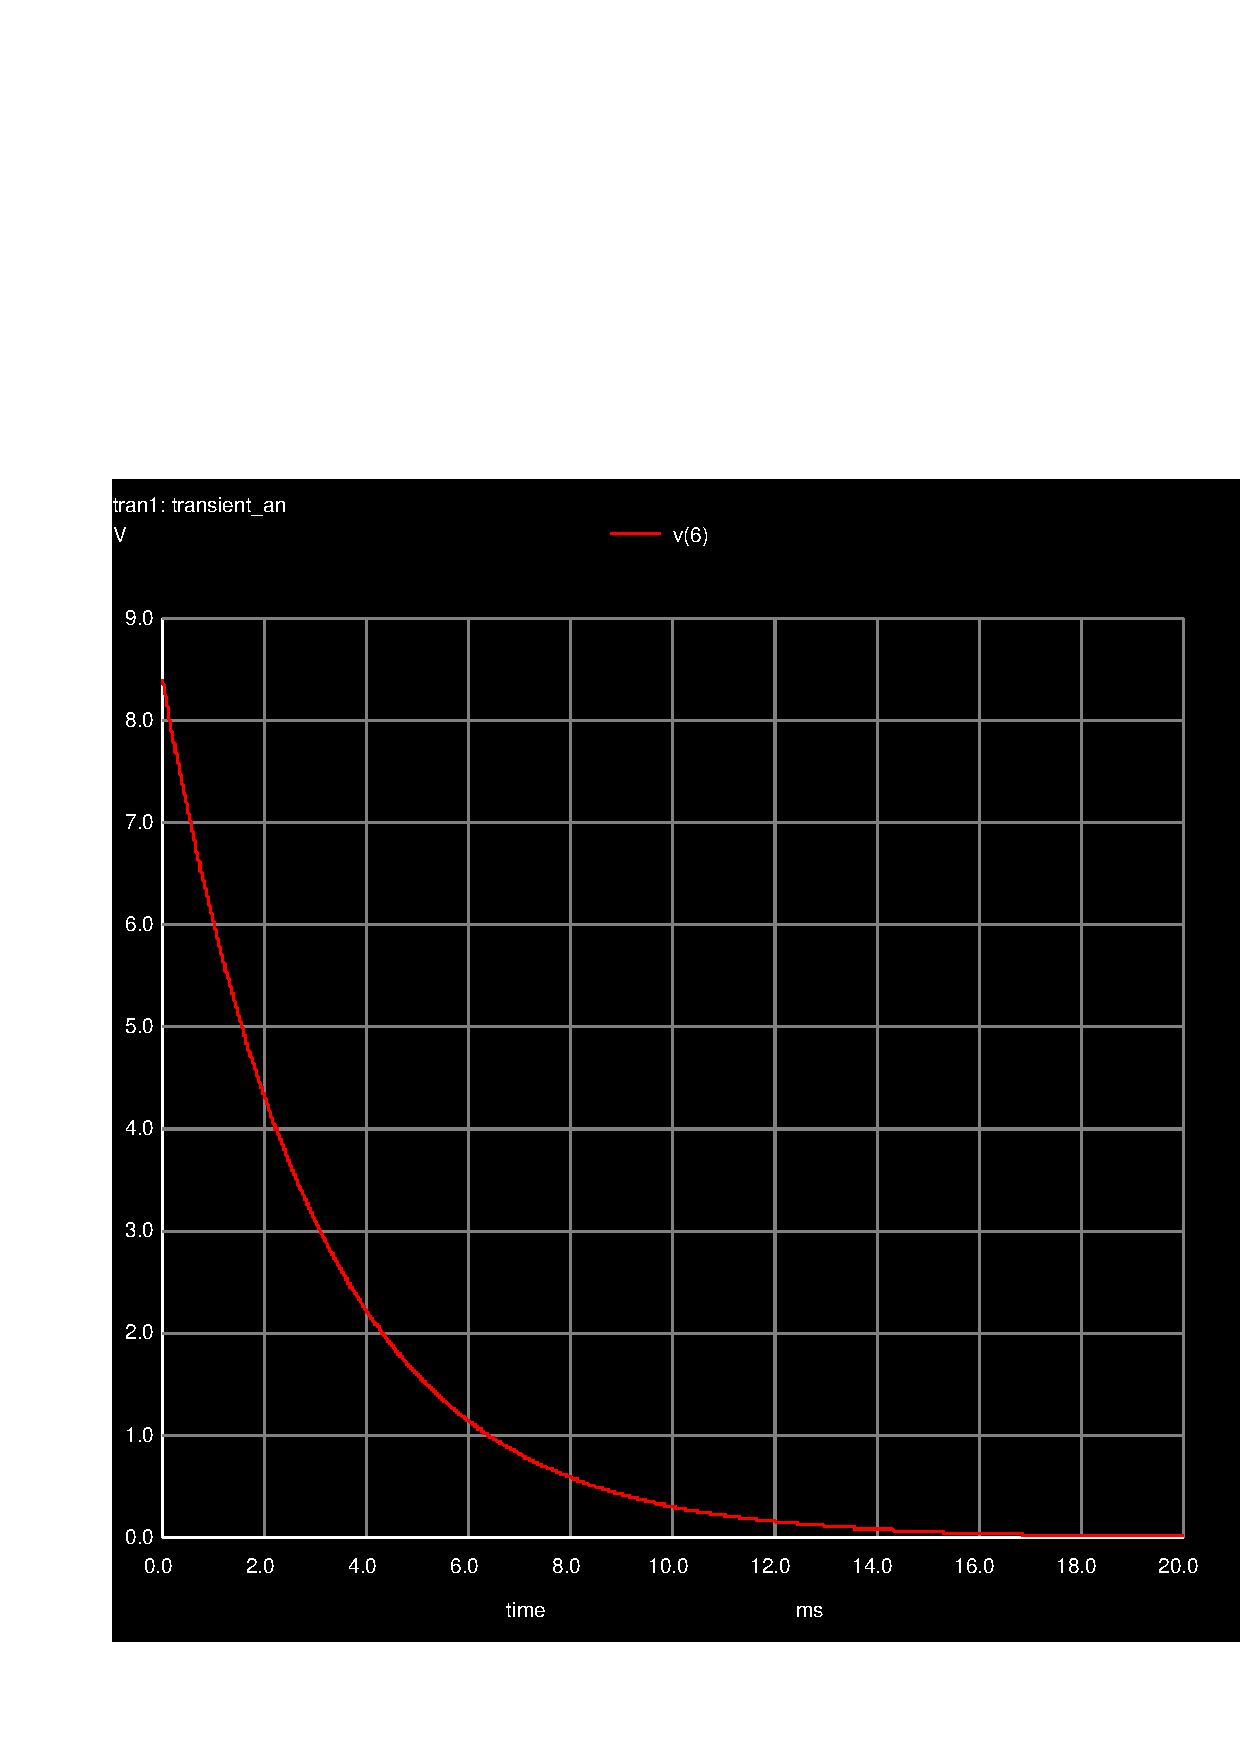
\includegraphics[width=.45\textwidth]{../sim/trans3.pdf} \label{fig:sim_nat} 
  } 
  \caption{Natural solution for voltage in node 6 for $t=[0,20]$.} 
\end{figure}

The solution for the natural solution in node 6 appears to be exactly the same.

\begin{figure}[H]
\hspace{-10mm}
  \subfigure[Theoretical analysis]{% 
    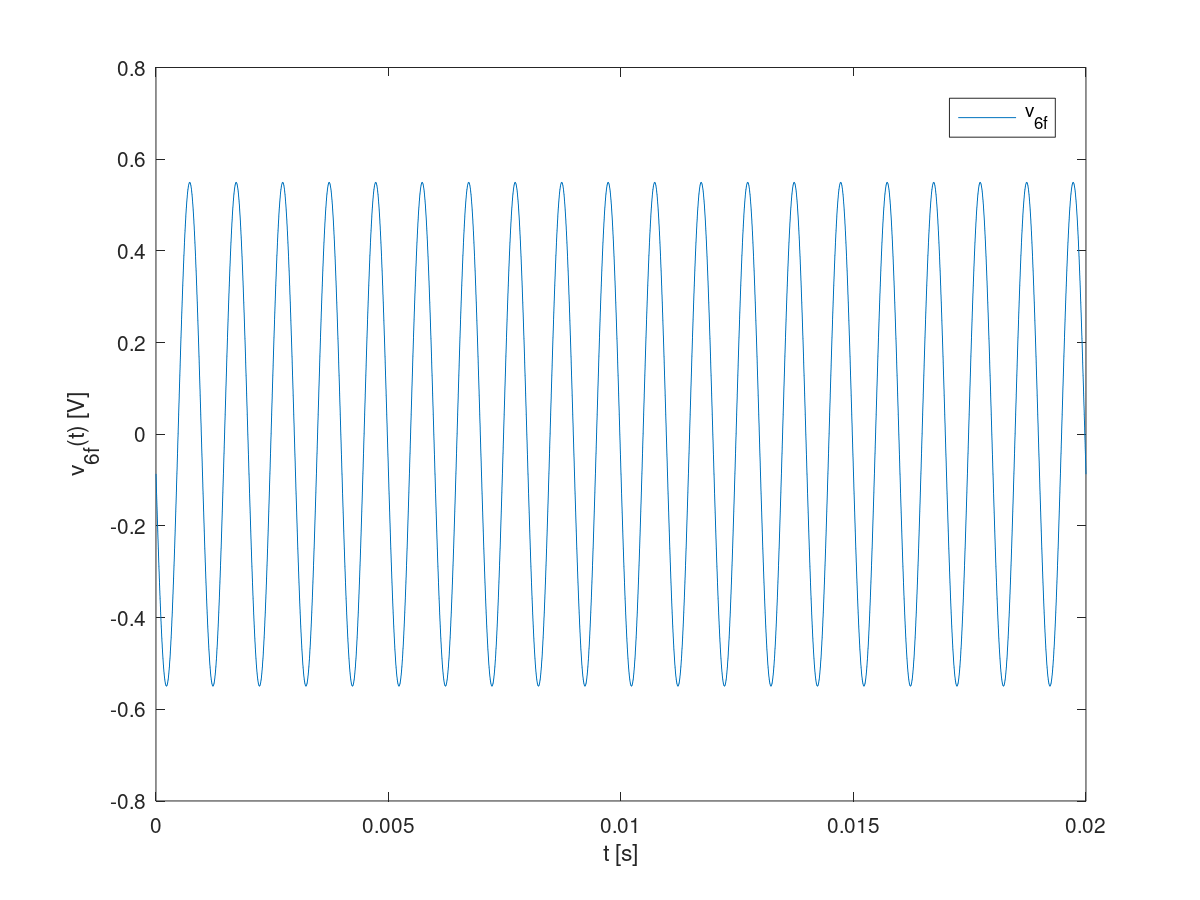
\includegraphics[width=.6\textwidth]{../mat/v6f.png} \label{fig:teo_for} 
  } 
  \subfigure[Simulation analysis]{% 
    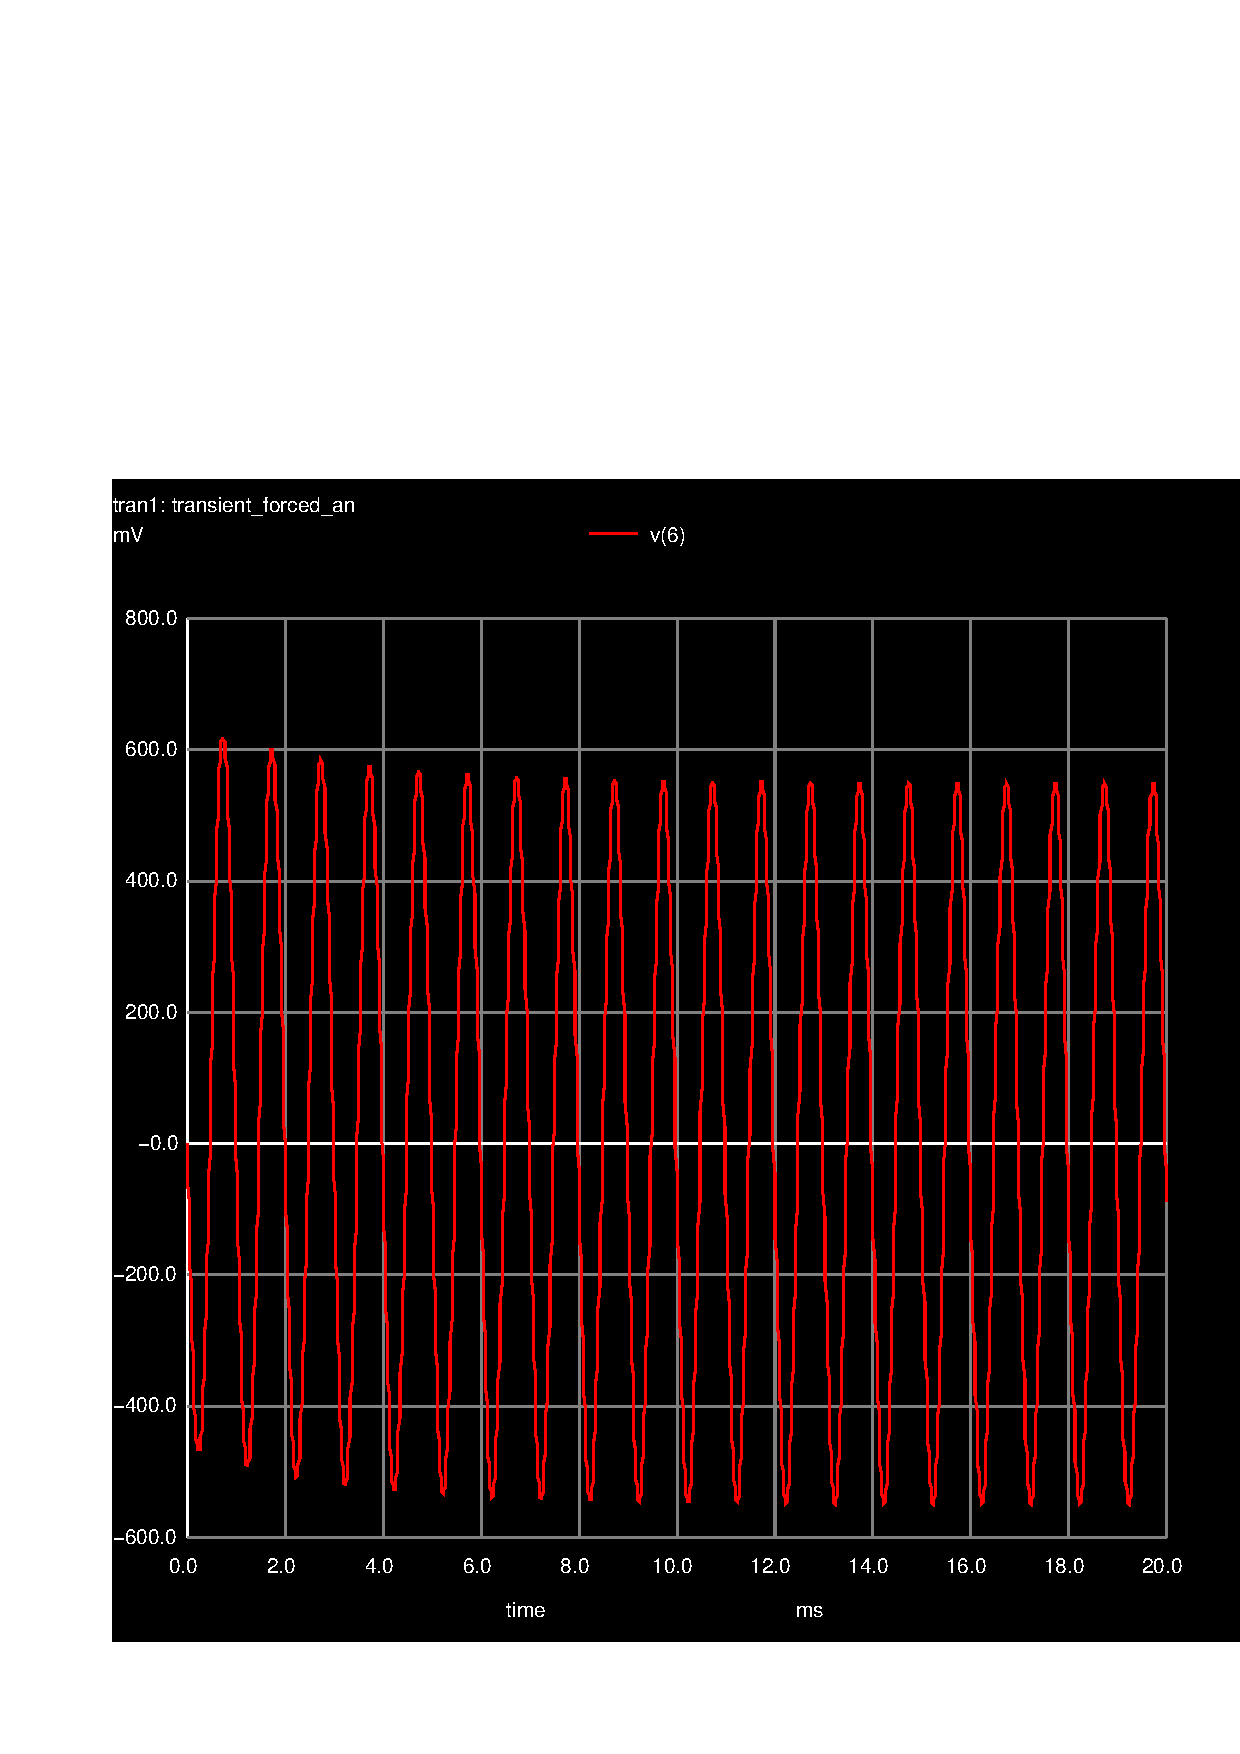
\includegraphics[width=.45\textwidth]{../sim/trans4.pdf} \label{fig:sim_for} 
  } 
  \caption{Forced solution for voltage in node 6 for $t=[0,20]$.} 
\end{figure}

As mentioned before, the only difference found between these 2 solution is that in the forced solution a small offset seems to exist in the first moments of the oscillation, but appears to stabilize on the expected solution.

\begin{figure}[H]
\hspace{-10mm}
  \subfigure[Theoretical analysis]{% 
    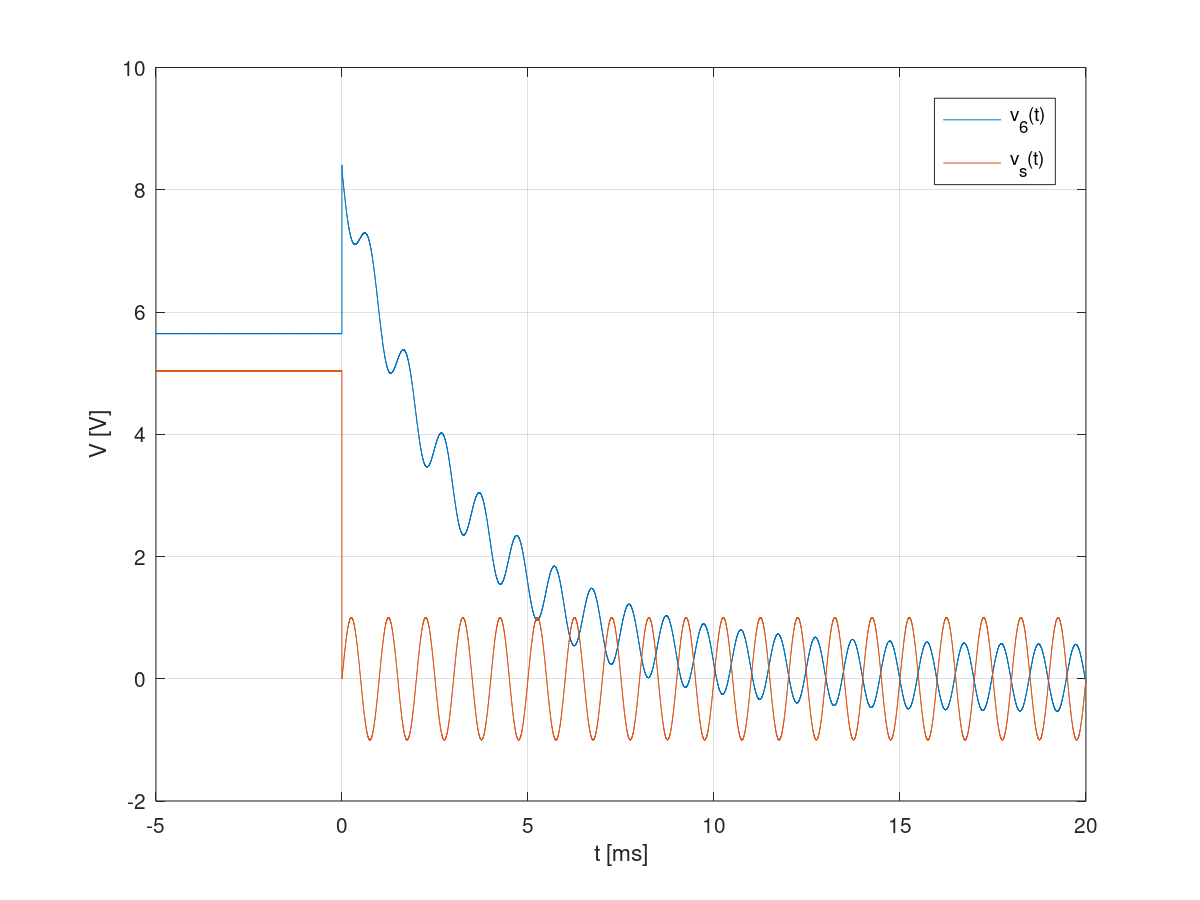
\includegraphics[width=.6\textwidth]{../mat/v6totsze.png} \label{fig:teo_comp} 
  } 
  \subfigure[Simulation analysis]{% 
    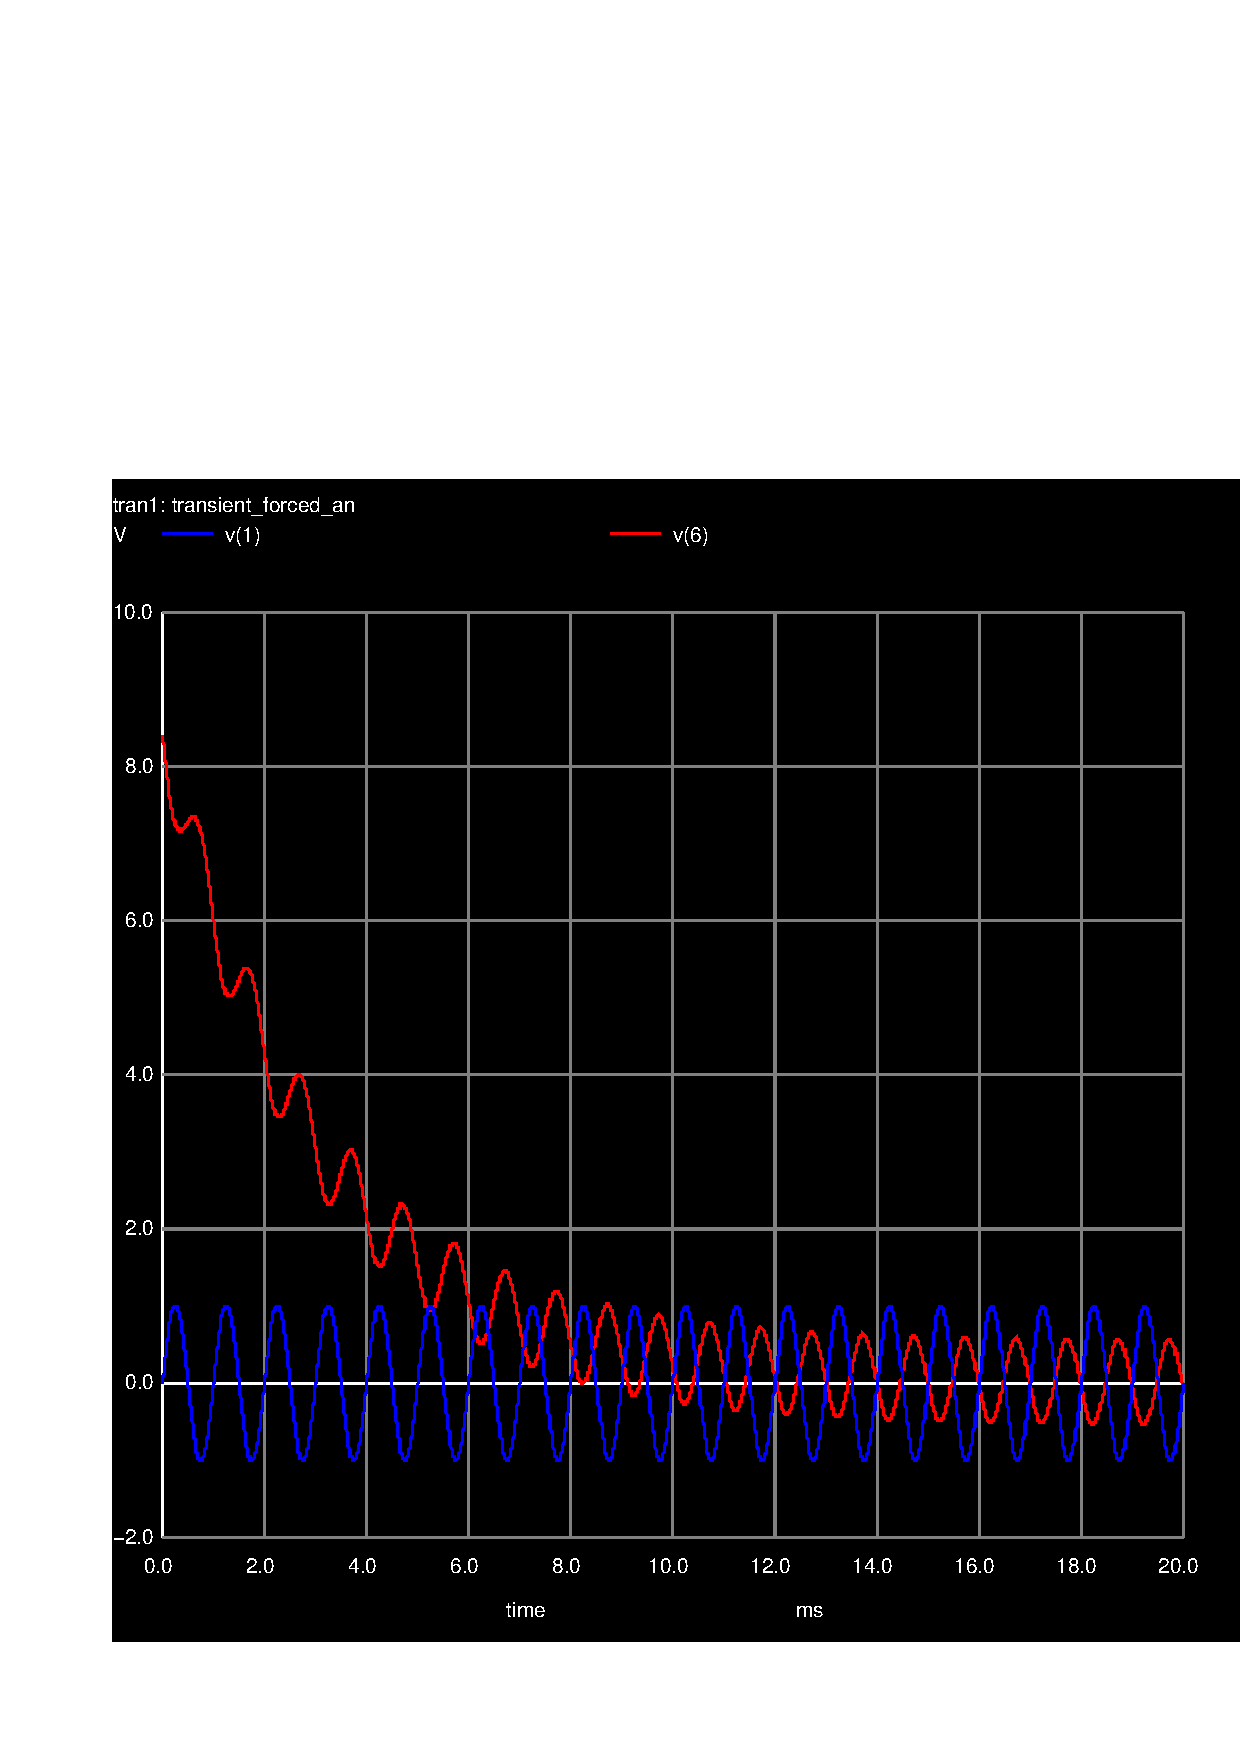
\includegraphics[width=.45\textwidth]{../sim/trans5.pdf} \label{fig:sim_comp} 
  } 
  \caption{Complete solution for voltage in node 6 for $t=[-5,20]$ and $t=[0,20]$.} 
\end{figure}

Besides the part of the forced solution that is now impossible to notice, the plots looks identical even in close inspection.

\begin{figure}[H]
\hspace{-10mm}
  \subfigure[Theoretical analysis]{% 
    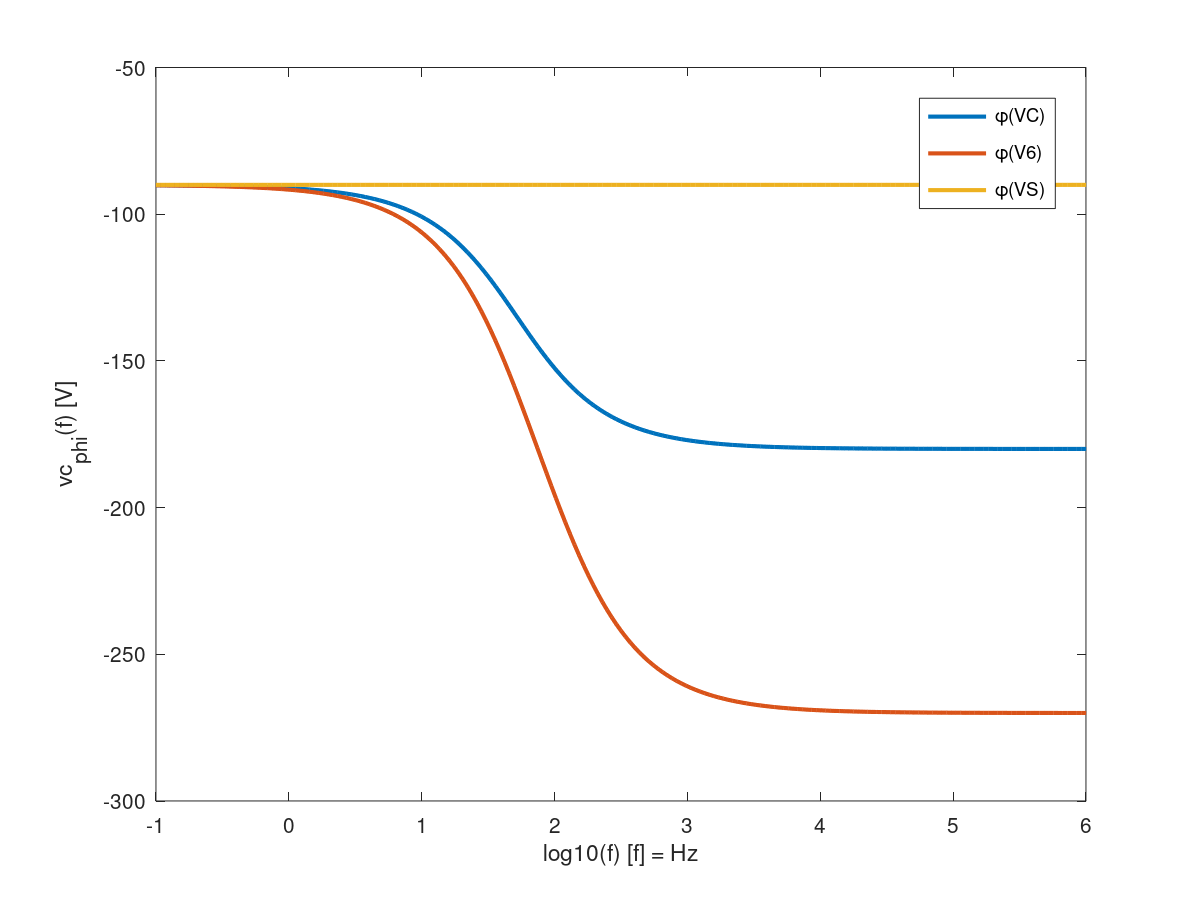
\includegraphics[width=.6\textwidth]{../mat/vcphi.png} \label{fig:teo_phi} 
  } 
  \subfigure[Simulation analysis]{% 
    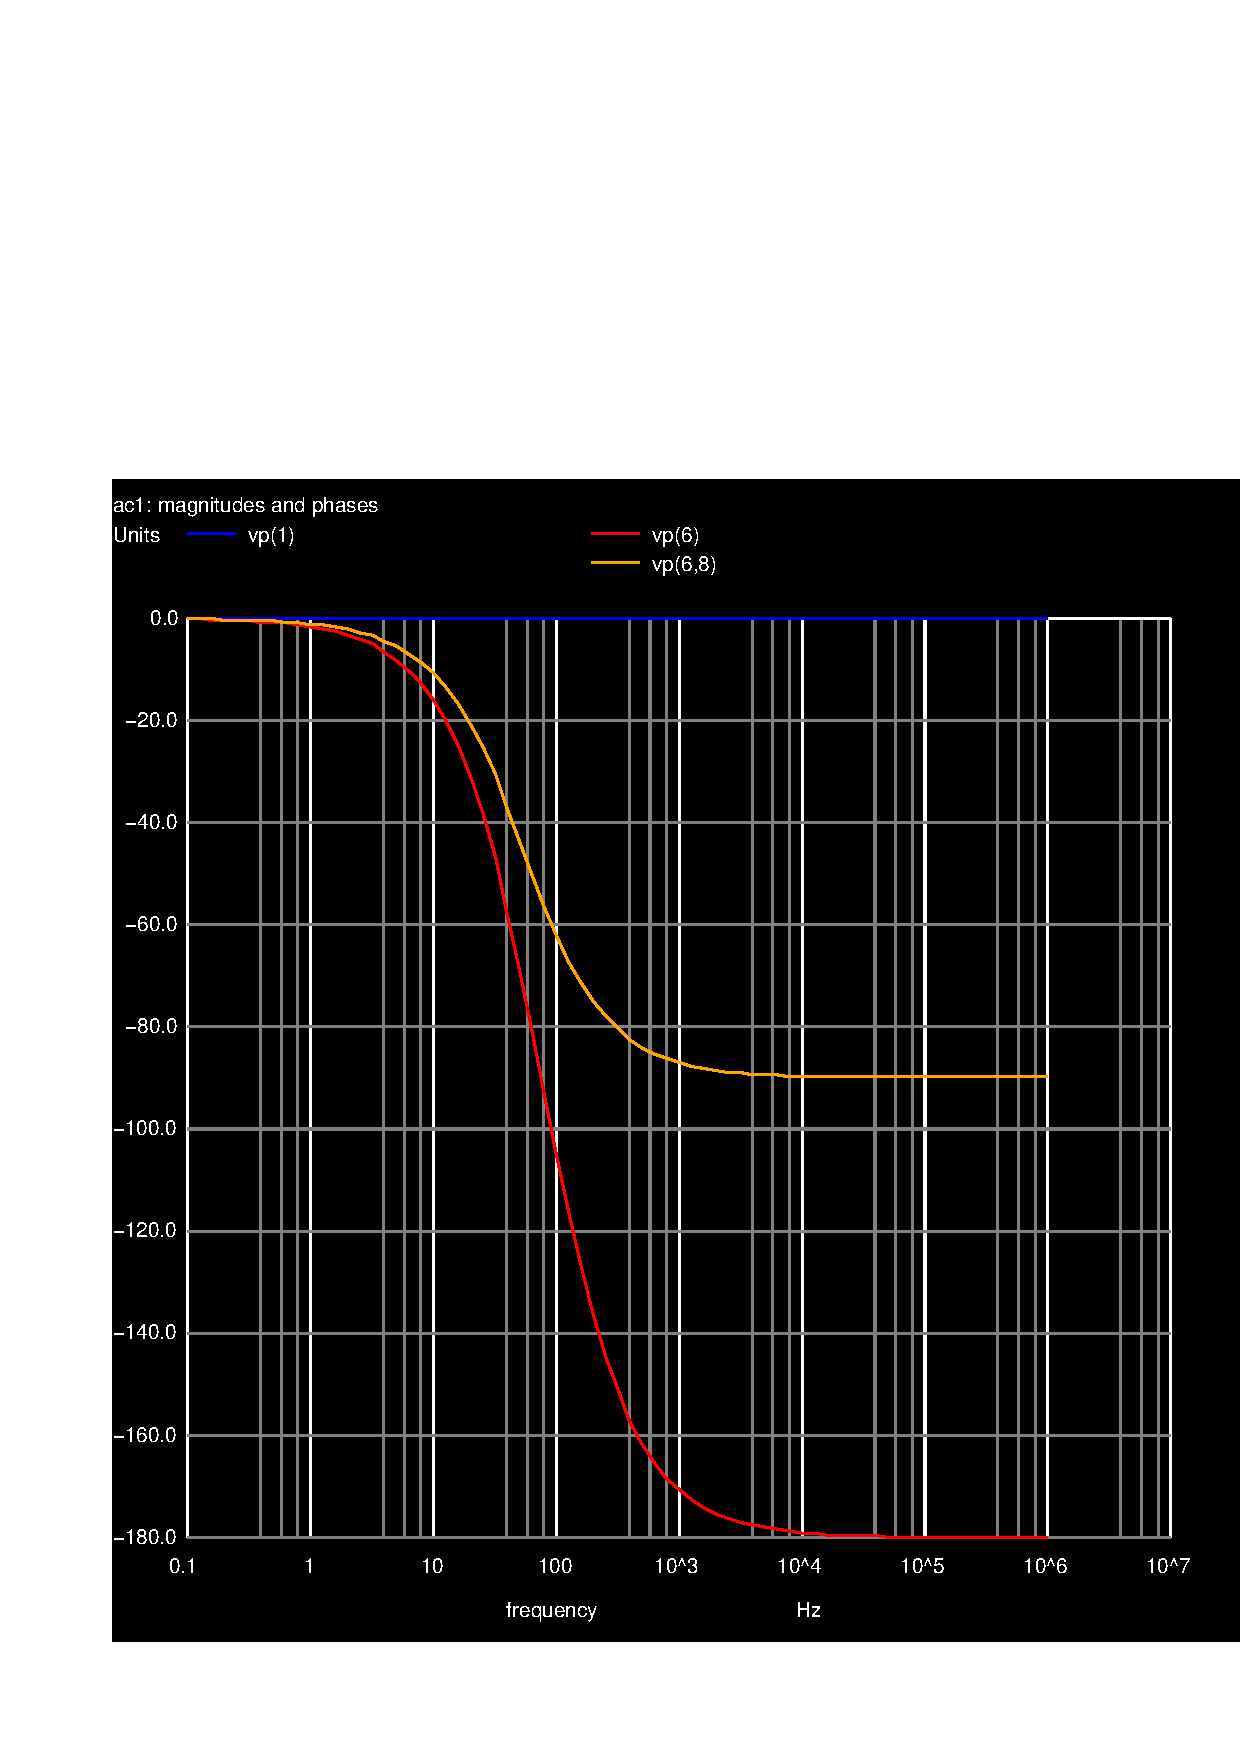
\includegraphics[width=.45\textwidth]{../sim/zezoca.pdf} \label{fig:sim_phi} 
  } 
  \caption{Phase difference as a function of the frequency of the voltage source.} 
\end{figure}

As mentioned before the same transition to a phase difference of a quarter and half a period is seen but \textit{Ngspice} automatically offsets the phases in order for the source to be at 0 degrees.


\begin{figure}[H]
\hspace{-10mm}
  \subfigure[Theoretical analysis]{% 
    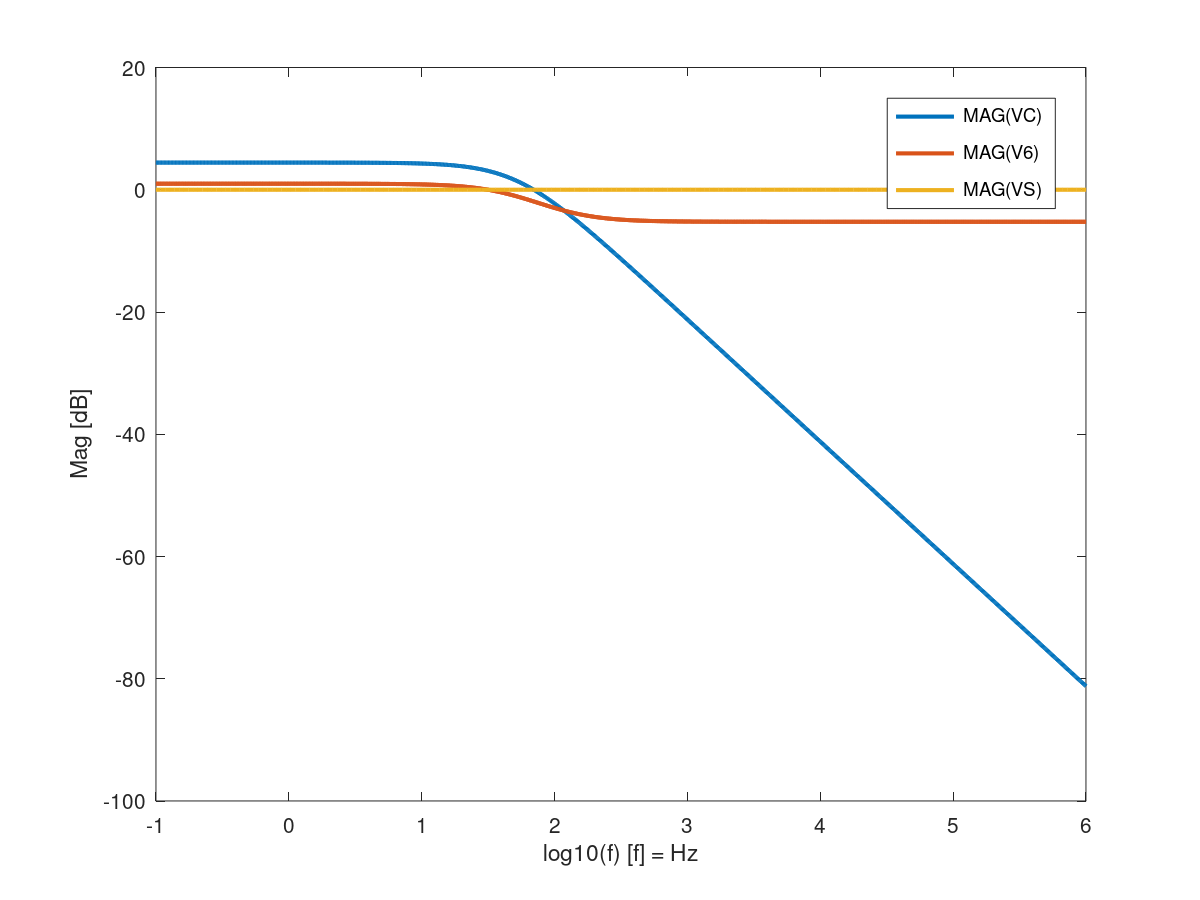
\includegraphics[width=.6\textwidth]{../mat/vcmag.png} \label{fig:teo_mag} 
  } 
  \subfigure[Simulation analysis]{% 
    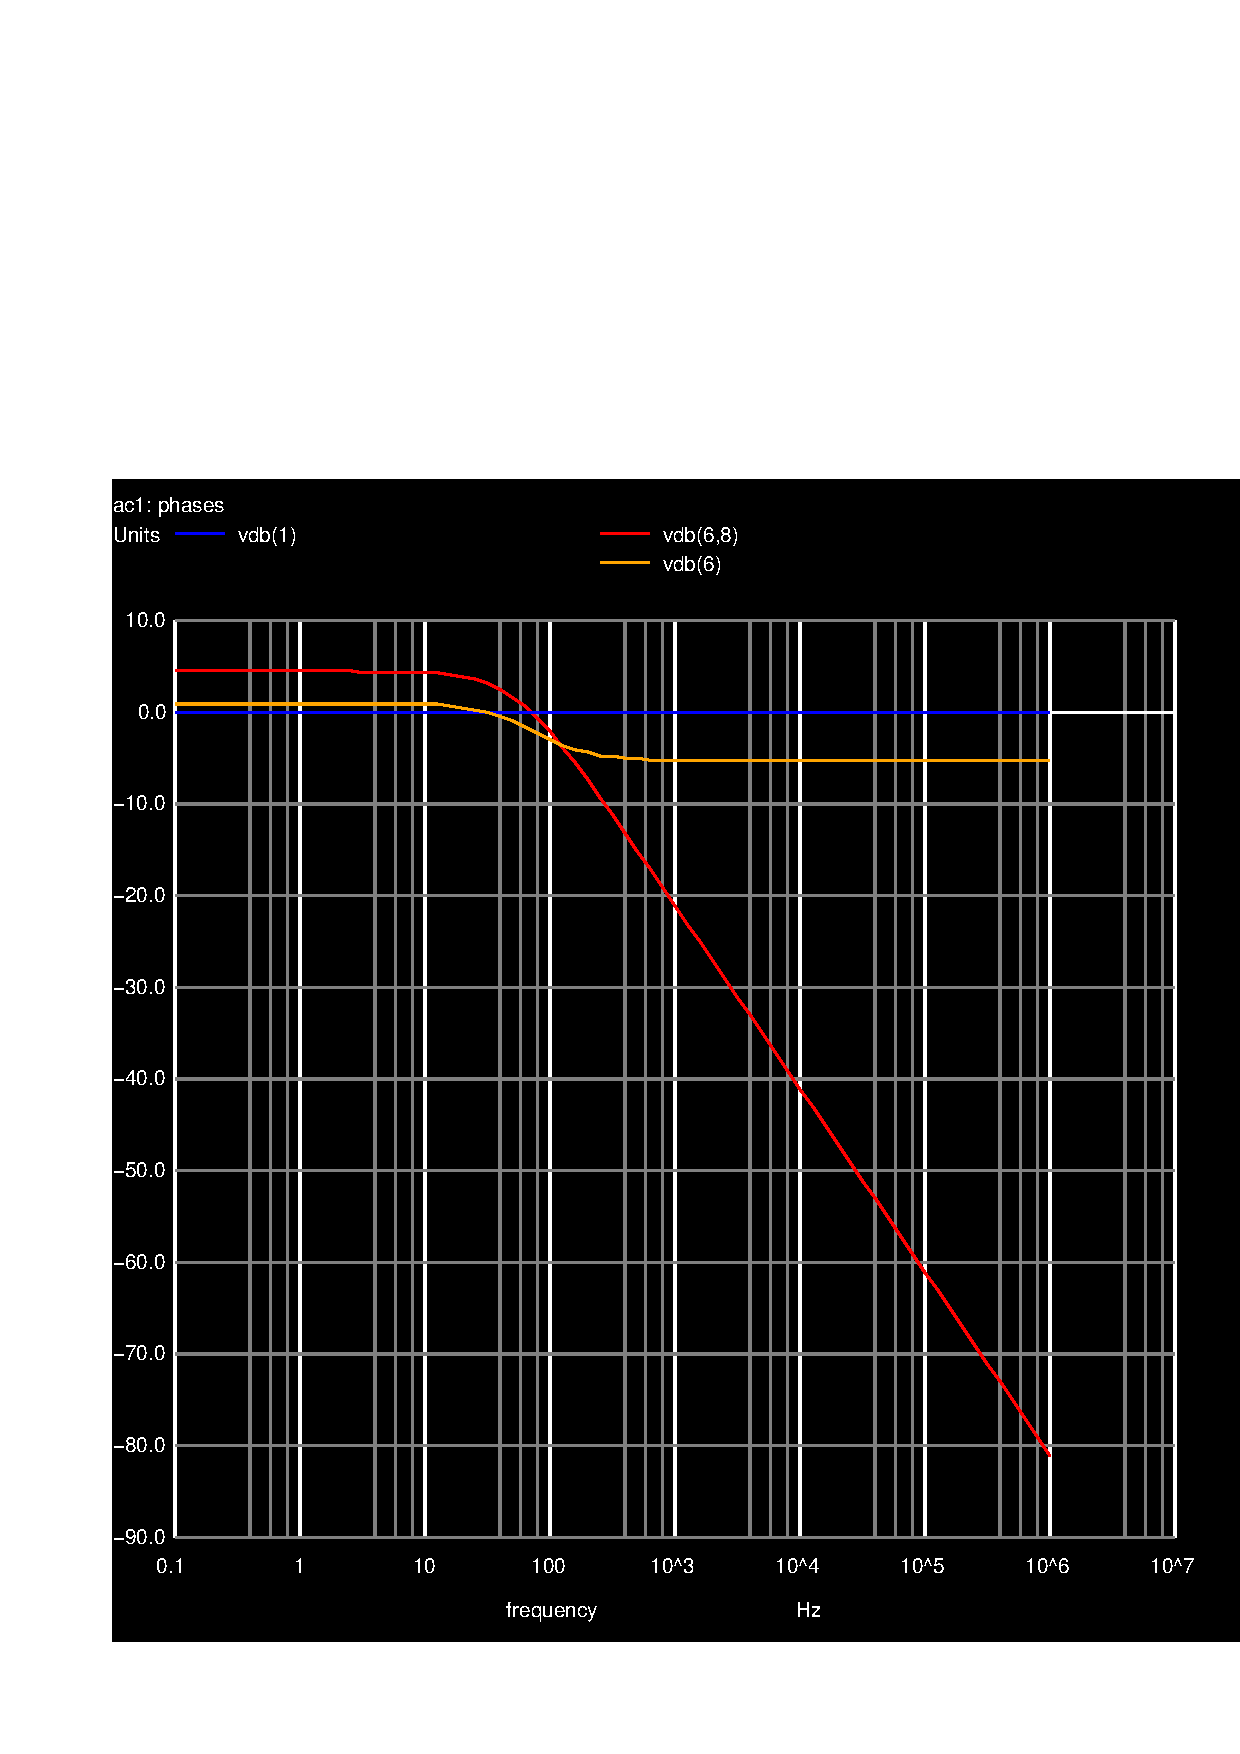
\includegraphics[width=.45\textwidth]{../sim/voltage_mag.pdf} \label{fig:sim_mag} 
  } 
  \caption{Magnitude as a function of the frequency of the voltage source.} 
  Once again no differences can be found between the 2 plots.
  
\end{figure}